%Ogata 29 do pdf (digrma de blocos na pag 32); Dorf 165 do pdf
A representação de um sistema dinâmico linear no espaço de estados descreve um sistema a partir das seguintes equações :
\begin{center}\label{eq:k1}
$\dot{x}=Ax+Bu$ \\
$y=Cx+Du$
\end{center}
em que $A$ é a matriz de estados, $B$ a matriz de entrada, $C$ a matriz de saída, $D$ a matriz de transmissão direta, $x$ é o vetor de variáveis de estado, $u$ o vetor de entradas e $y$ o vetor de saídas. A Figura \ref{fig:ss_diagram} exibe um diagrama de blocos para a representação em espaço de estados definida.

\begin{figure}[!htb]
    \centering
    \caption{Diagrama de blocos de um sistema linear e contínuo tempo representado no espaço de estados}
    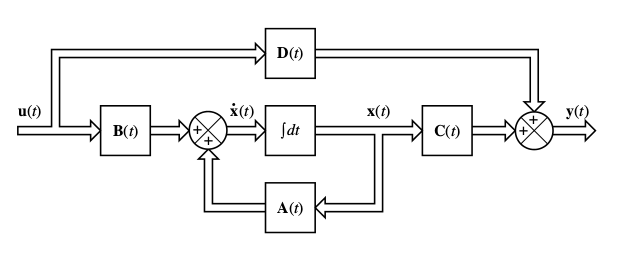
\includegraphics[width=0.9\textwidth]{./04-figuras/fund_teorica/ss_diagram}
    \fonte{\citeonline[p.~32]{Ogata2010}}
    \label{fig:ss_diagram}
\end{figure}

%A representação no espaço de estados oferece uma ferramenta poderosa para a manipulação da representação do sistema, permitindo que as variáveis de estado sejam representadas de forma independente entre si a partir do processo de desacoplamento delas.
%
%O processo de desacoplamento de variáveis de estado é baseado em ferramentas matemáticas aplicando manipulações sobre frações parciais. A partir deste processo, por exemplo, o sistema mostrado na Figura \ref{fig:ss_coupled}, que representa um sistema de controle de um motor CC com velocidade como saída e é representado pela função de transferência:
%\begin{equation}
%G(s)=\frac{30(s+1)}{(s+5)(s+2)(s+3)}
%\end{equation}
%pode ser representado por uma função de transferência do tipo:
%\begin{equation}
%G(s)=\frac{q(s)}{(s-s_1)(s-s_2)(s-s_3)}
%\end{equation}
%cuja resposta é ditada por $s_1$, $s_2$ e $s_3$. Utilizando a expansão de frações parciais, pode-se representar a mesma função de transferência por \cite[p.~183]{Dorf2011}:
%\begin{equation}
%T(s)=\frac{k_1}{s+5}+\frac{k_2}{s+2}+\frac{k_3}{s+3}
%\end{equation}
%
%\begin{figure}[!htb]
%    \centering
%    \caption{Diagrama de blocos representando o controle de um motor CC com velocidade como saída}
%    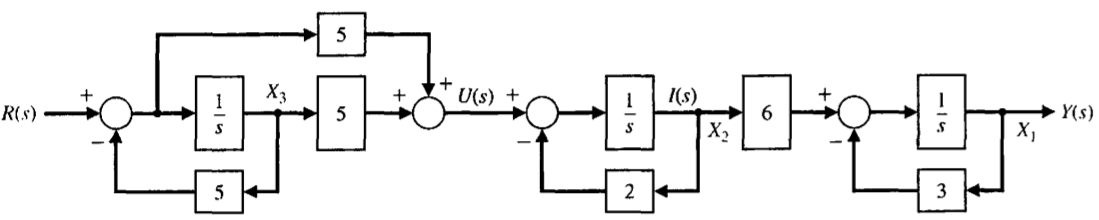
\includegraphics[width=1\textwidth]{./04-figuras/fund_teorica/ss_coupled_blocks}
%    \fonte{\citeonline[p.~182]{Dorf2011}}
%    \label{fig:ss_coupled}
%\end{figure}
%
%A partir de manipulações matemáticas relacionadas à expansão de frações parciais, constata-se que $k_1=-20$, $k_2=-10$ e $k_3=30$ \cite[p.~182]{Dorf2011}. Com isto, o sistema exibido na Figura \ref{fig:ss_coupled} pode ser representado como mostrado na Figura \ref{fig:ss_decoupled} que, como se pode ver, trata $X_1$, $X_2$ e $X_3$ de forma completamente independente e somando suas respectivas contribuições em $Y(s)$. Desta forma, pode-se ver claramente como cada variável de estado contribui para a saída ($Y(s)$) a partir de uma dada entrada ($X(s)$).
%
%\begin{figure}[!htb]
%    \centering
%    \caption{Diagrama de blocos representando o controle de um motor CC com velocidade como saída e implementando desacoplamento das variáveis de estado}
%    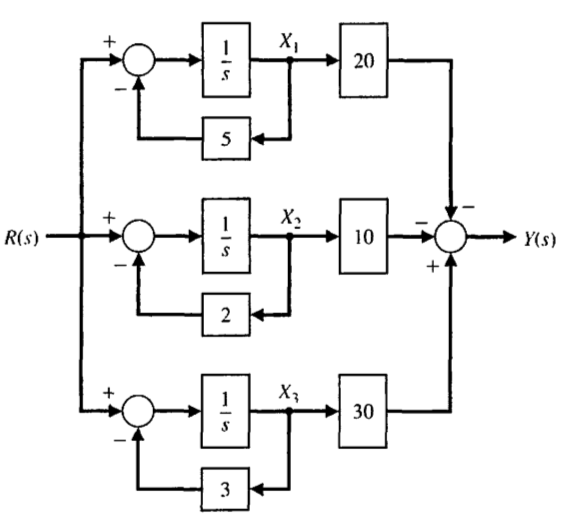
\includegraphics[width=0.6\textwidth]{./04-figuras/fund_teorica/ss_decoupled_blocks}
%    \fonte{\citeonline[p.~182]{Dorf2011}}
%    \label{fig:ss_decoupled}
%\end{figure}








